% Welcome! This is the unofficial University of Udine beamer template.

% See README.md for more informations about this template.

% This style has been developed following the "Manuale di Stile"
% (Style Manual) of the University of Udine. You can find the
% manual here: https://www.uniud.it/it/ateneo-uniud/ateneo-uniud/identita-visiva/manuali-immagine-stile/manuale-stile

% Note: for some reason, the RGB values specified in the manual
% do NOT render correctly in Beamer, so they have been redefined
% for this document using the high level chromo-optic deep neural 
% quantistic technology offered by Microsoft Paint's color picker.

% We defined four theme colors: UniBrown, UniBlue, UniGold
% and UniOrange. For example, to write some uniud-brownish
% text, just use: \textcolor{UniBrown}{Hello!}

% Note that [usenames,dvipsnames] is MANDATORY due to compatibility
% issues between tikz and xcolor packages.

\documentclass[usenames,dvipsnames]{beamer}
\usepackage[utf8]{inputenc}
\usepackage{verbatim}
%\usetheme{./beamer_style/uniud}
\usepackage{amsmath}
\usepackage{graphicx}
\usepackage{caption}
\usepackage{enumitem}
\usepackage{multirow}
\usepackage[flushleft]{threeparttable}
\usepackage{tabularx, makecell, booktabs}
\captionsetup{font=footnotesize}
\usepackage{mathtools}
\usepackage[numbers,sort]{natbib}
\usepackage{./beamer_style/beamerthemeuniud}

\setbeamertemplate{caption}[numbered]

\DeclarePairedDelimiterX{\infdivx}[2]{[}{]}{%
  #1\;\delimsize\|\;#2%
}

\makeatletter
\DeclareRobustCommand{\abs}{\@ifstar\star@abs\normal@abs}
\newcommand{\star@abs}[1]{\left|#1\right|}
\newcommand{\normal@abs}[2][]{\mathopen{#1|}#2\mathclose{#1|}}
\makeatother


% Beamer files path
%\makeatletter
%\def\beamer@themefile{beamer_style/beamerthemeuniud.sty}
%\def\beamer@themelocpath{beamer_style}
%\makeatother

%%% Bibliography
%\usepackage[style=authoryear,backend=biber]{biblatex}
%\addbibresource{bibliography.bib}


% Author names in publication list are consistent 
% i.e. name1 surname1, name2 surname2
% See https://tex.stackexchange.com/questions/106914/biblatex-does-not-reverse-the-first-and-last-names-of-the-second-author
%\DeclareNameAlias{author}{first-last}

%%% Suppress biblatex annoying warning
\usepackage{silence}
\WarningFilter{biblatex}{Patching footnotes failed}

%%% Some useful commands
% pdf-friendly newline in links
\newcommand{\pdfnewline}{\texorpdfstring{\newline}{ }} 
% Fill the vertical space in a slide (to put text at the bottom)
\newcommand{\framefill}{\vskip0pt plus 1filll}

% Define a custom bullet command with color and size
%\newcommand{\mybullet}{\textcolor{UniGold}{\rule{6px}{6px}}}

% Define a custom itemize style with custom bullets
\setlist[itemize]{
  label=\textcolor{UniGold}{$\bullet$}, % Use the custom bullet command
  left=0pt,        % Adjust left margin if needed
  itemsep=6pt,     % Adjust spacing between items
}

\title[Generative AI in Healthcare]{\textcolor{SupeGrayDark}{Generative AI in Healthcare: Applications and Evaluation of Effectiveness}}
\date{\textcolor{SupeGrayDark}{Dec 13, 2024}}
\author[Lorenzo Zanolin]{
  \parbox{0.45\linewidth}{
    \textcolor{SupeGrayDark}{
      \textbf{Candidate:}\\ Lorenzo Zanolin\\
      %\texttt{zanolin.lorenzo@spes.uniud.it}
    }
  }
  \hfill
  \parbox{0.45\linewidth}{
    \textcolor{SupeGrayDark}{
      \textbf{Supervisor:}\\ Prof. Giuseppe Serra\\
      \textbf{Co-Supervisor:}\\ Prof. Jan Steinbrener
    }
  }
}
\institute{\textcolor{SupeGrayDark}{Artificial Intelligence \& Cybersecurity}}

\begin{document}

\begin{frame}
\titlepage
\end{frame}

\begin{frame}{Background \& Motivations}
  
  \only<1->{\textbf{Background}\\
  \begin{itemize}
    \item Generative AI \textit{goal}: derive a probability distribution from data to generate new synthetic data.
    \item \textit{Masked Multi-Head Self Attention}: captures global dependencies, process sequences in parallel and generates embeddings that improve performance on a wide range of tasks.
  \end{itemize}}
  \vspace{4mm}
  \uncover<2->{\textbf{Motivations}\\
  \begin{itemize}
    \item Generative AI can be integrated within workflows to help clinicians.
    \item Absence of a complete evaluation framework in the literature $\rightarrow$ new framework that combines human feedback and metric based feedback.
  \end{itemize}}
\end{frame}

\begin{frame}{Platform \& Components}
  
  \only<1->{\textbf{Salesforce}\\
  \begin{itemize}
    \item Enables companies to manage relationships with customers, prospects and employees through customizable interaction rules.
    \item Integrates with modules such as Health Cloud and Einstein.
  \end{itemize}}
  \vspace{5mm}
  \uncover<2->{\textbf{Einstein 1}\\
  \begin{itemize}
    \item Enables the use of genAI models within Salesforce.
    \item Allows for the creation of reusable prompts with database integration (RAG).
    \item Trust Layer framework to ensure data security during information exchange with LLMs.
  \end{itemize}}
\end{frame}

\begin{frame}{Einstein Trust Layer}
  
  \only<1>{
        \begin{figure}[b]
            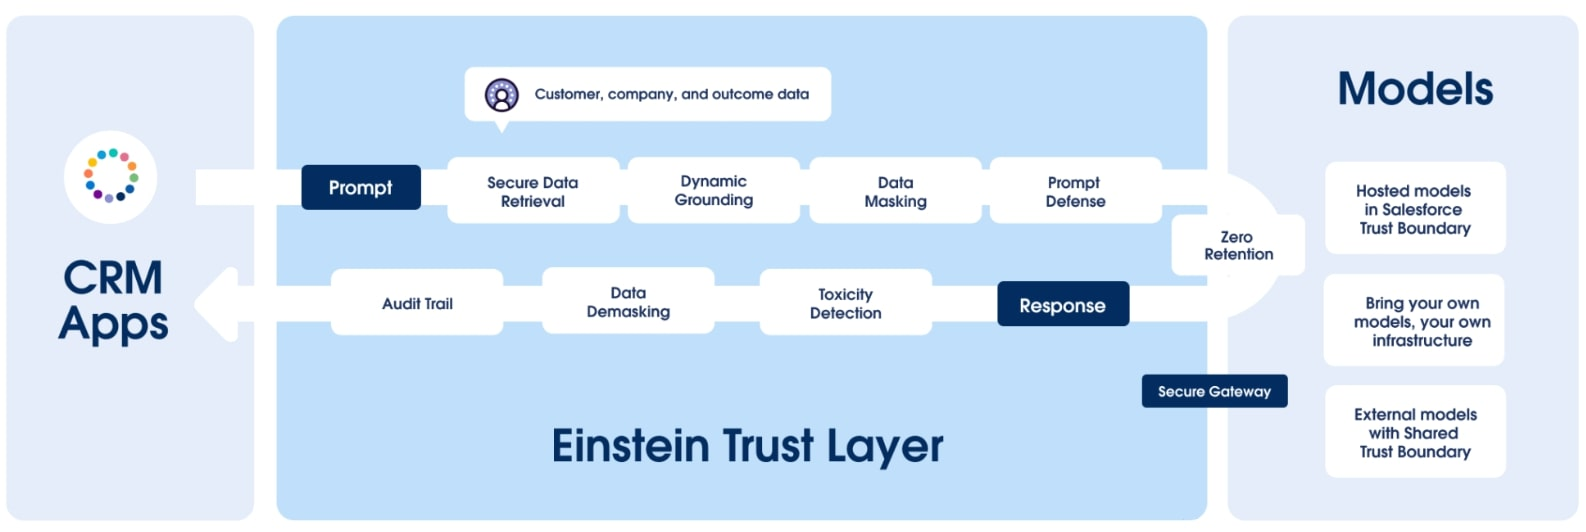
\includegraphics[scale=0.20]{images/TrustLayer1.jpg}
        \end{figure}}
    
    \only<2>{
        \begin{figure}[b]
            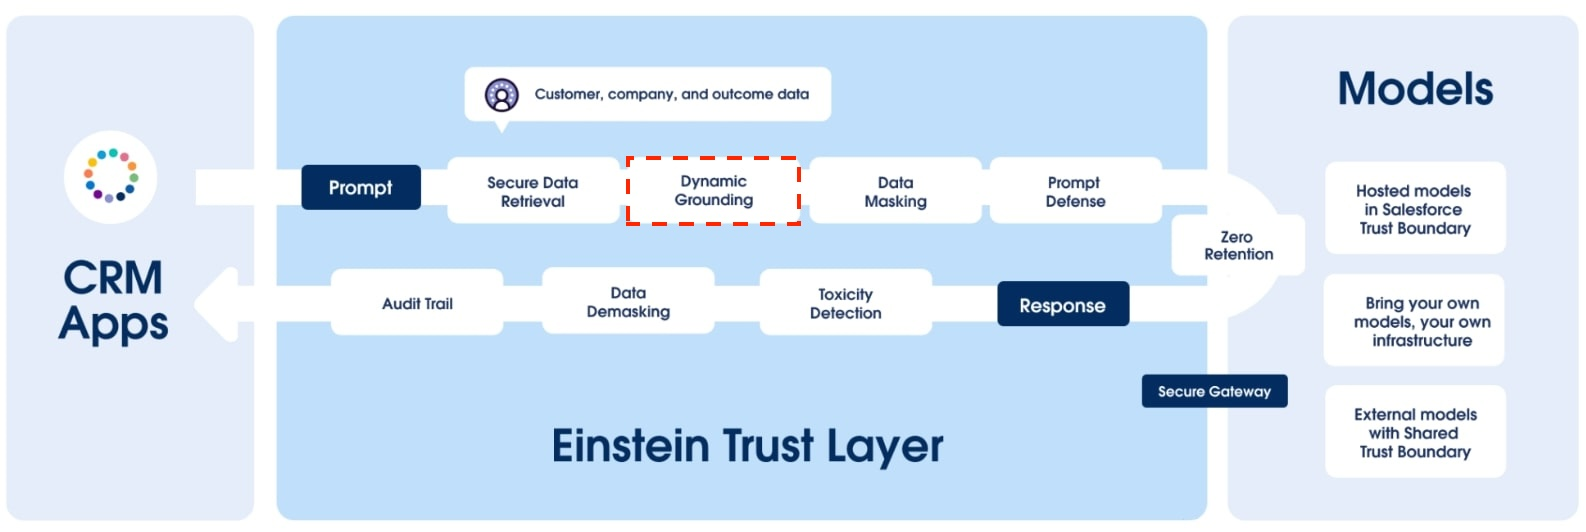
\includegraphics[scale=0.20]{images/TrustLayer2.jpg}
        \end{figure}}
  \only<3>{
        \begin{figure}[b]
            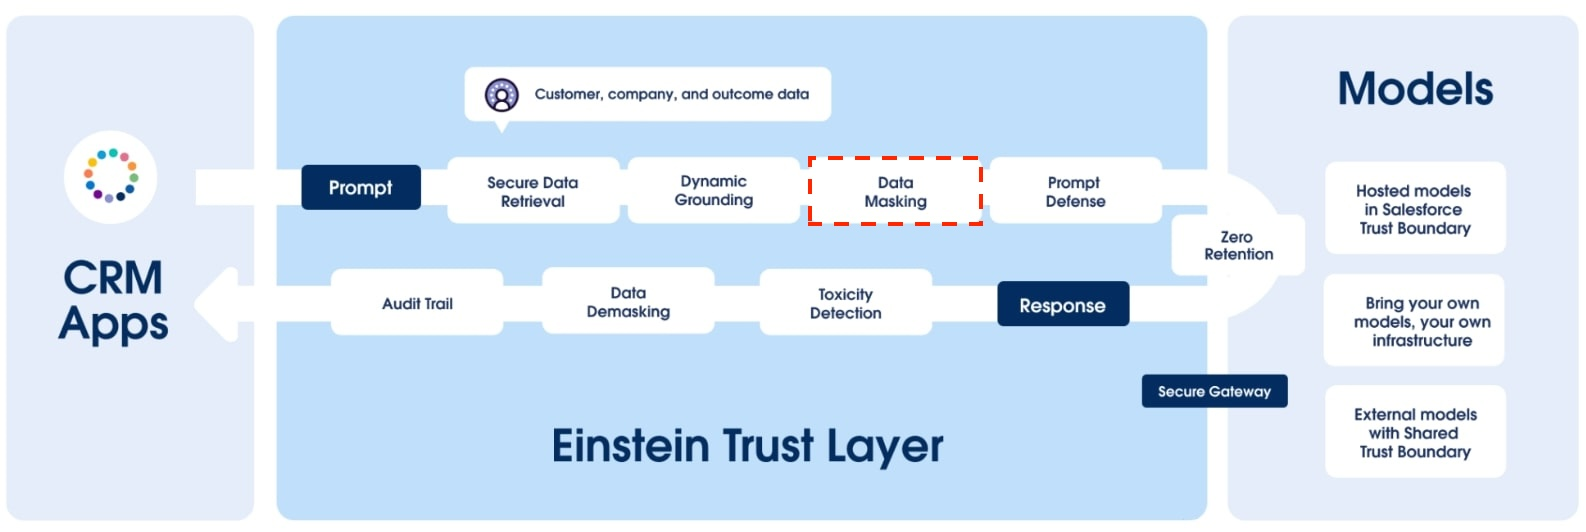
\includegraphics[scale=0.20]{images/TrustLayer3.jpg}
        \end{figure}}
    
    \only<4>{
        \begin{figure}[b]
            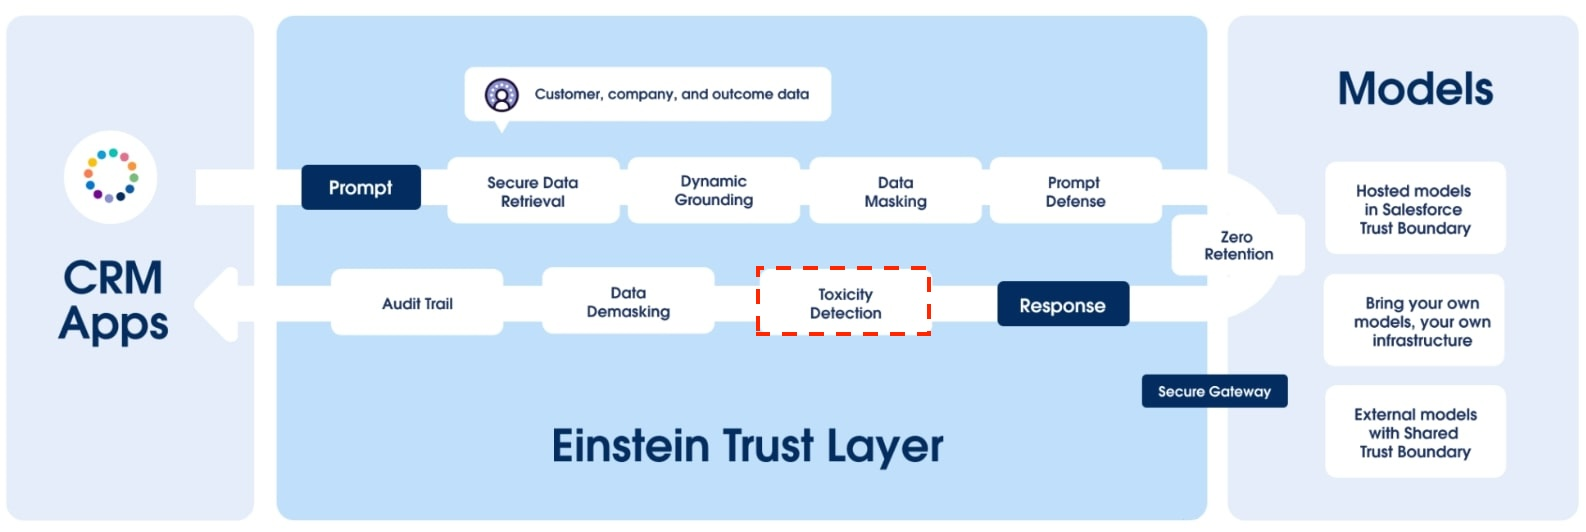
\includegraphics[scale=0.20]{images/TrustLayer5.jpg}
        \end{figure}}
  \only<5>{
        \begin{figure}[b]
            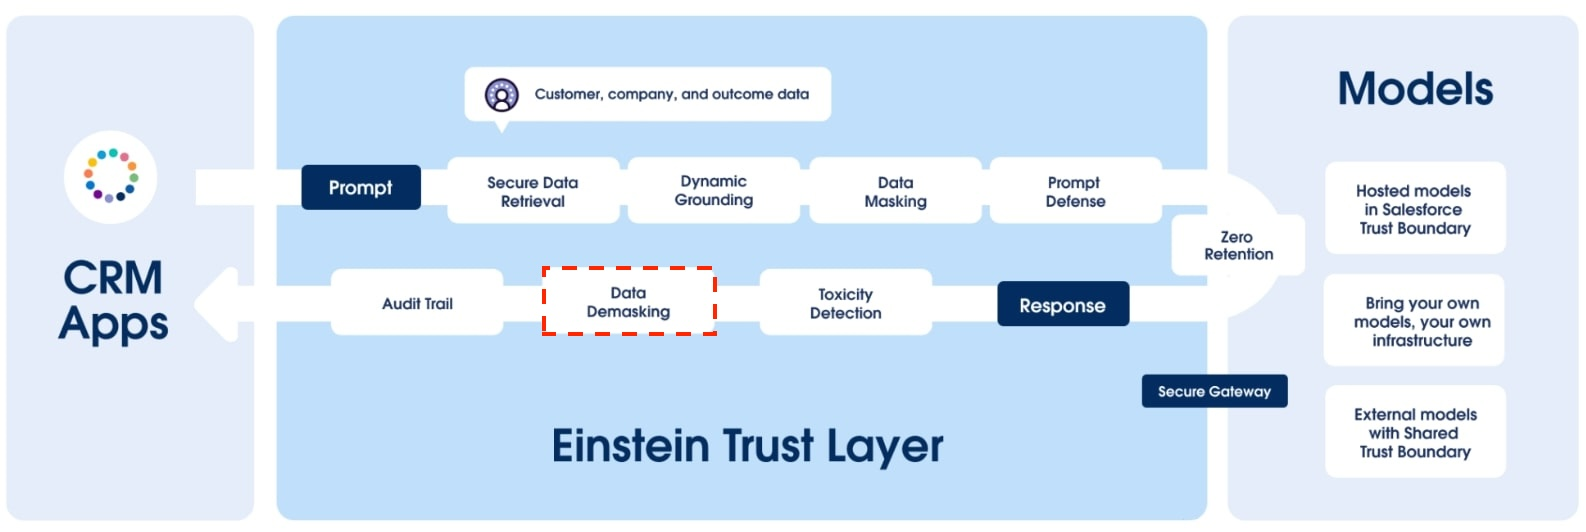
\includegraphics[scale=0.20]{images/TrustLayer4.jpg}
        \end{figure}}
\end{frame}

\begin{frame}{Use Case}
  
  \only<1->{\textbf{Health Clinic}\\
  \begin{itemize}
    \item Application intended for healthcare clinics that manage numerous patients and offer a wide range of services.
    \vspace{5mm}
    \item Tasks to be implemented with Copilot:
  }
  \uncover<2->{
    \begin{itemize}
      \item Patient Summary
  }

  \uncover<3->{
      \item List Possible Problems
  }

  \uncover<4->{
      \item Send Visit Details
    \end{itemize}
  \end{itemize}
  }
\end{frame}

\begin{frame}{Patient Summary}
  
  \only<1->{Invoked by the doctor before receiving the patient: quick and detailed overview of all the patient’s conditions.}

  \uncover<2->{\begin{figure}[b]
    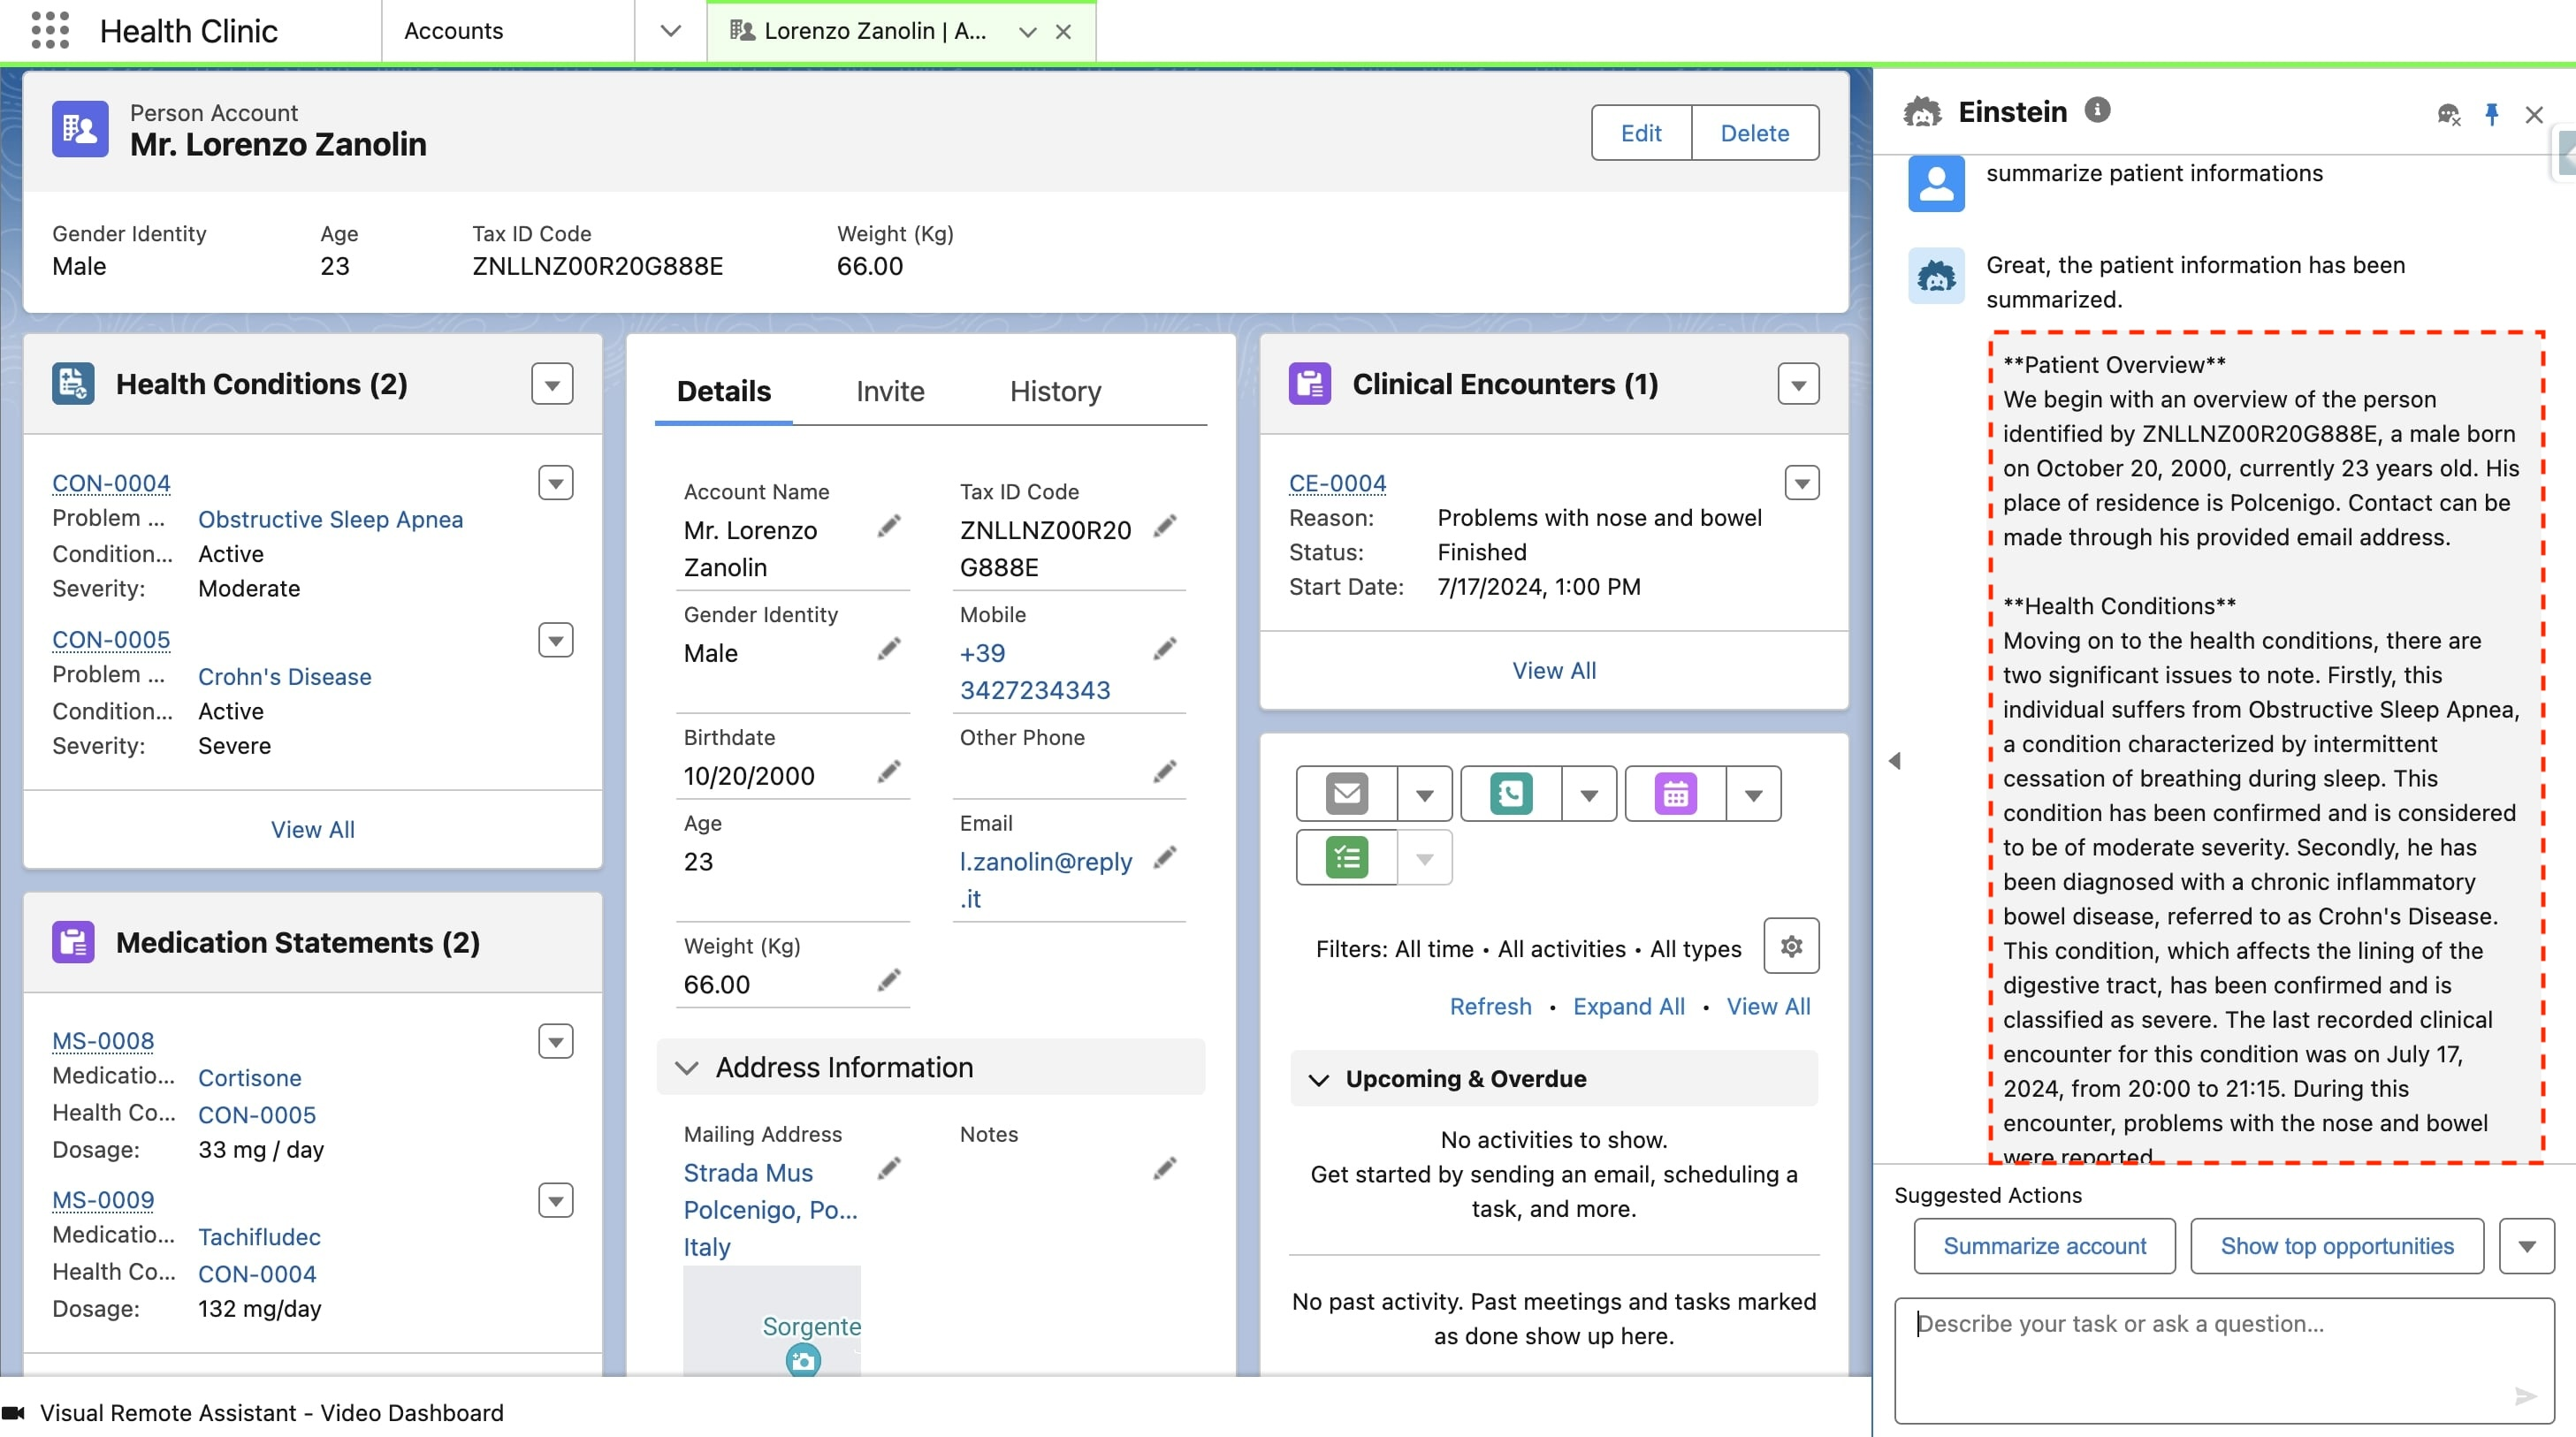
\includegraphics[scale=0.1]{images/SummarizePatient.jpg}
\end{figure}}
\end{frame}

\begin{frame}{List Possible Problems}
  
  \only<1->{Identifies potential conditions based on the patient’s symptoms, providing a list of possible diagnoses and medications, with dosage calculations for of them.}

  \uncover<2->{\begin{figure}[b]
    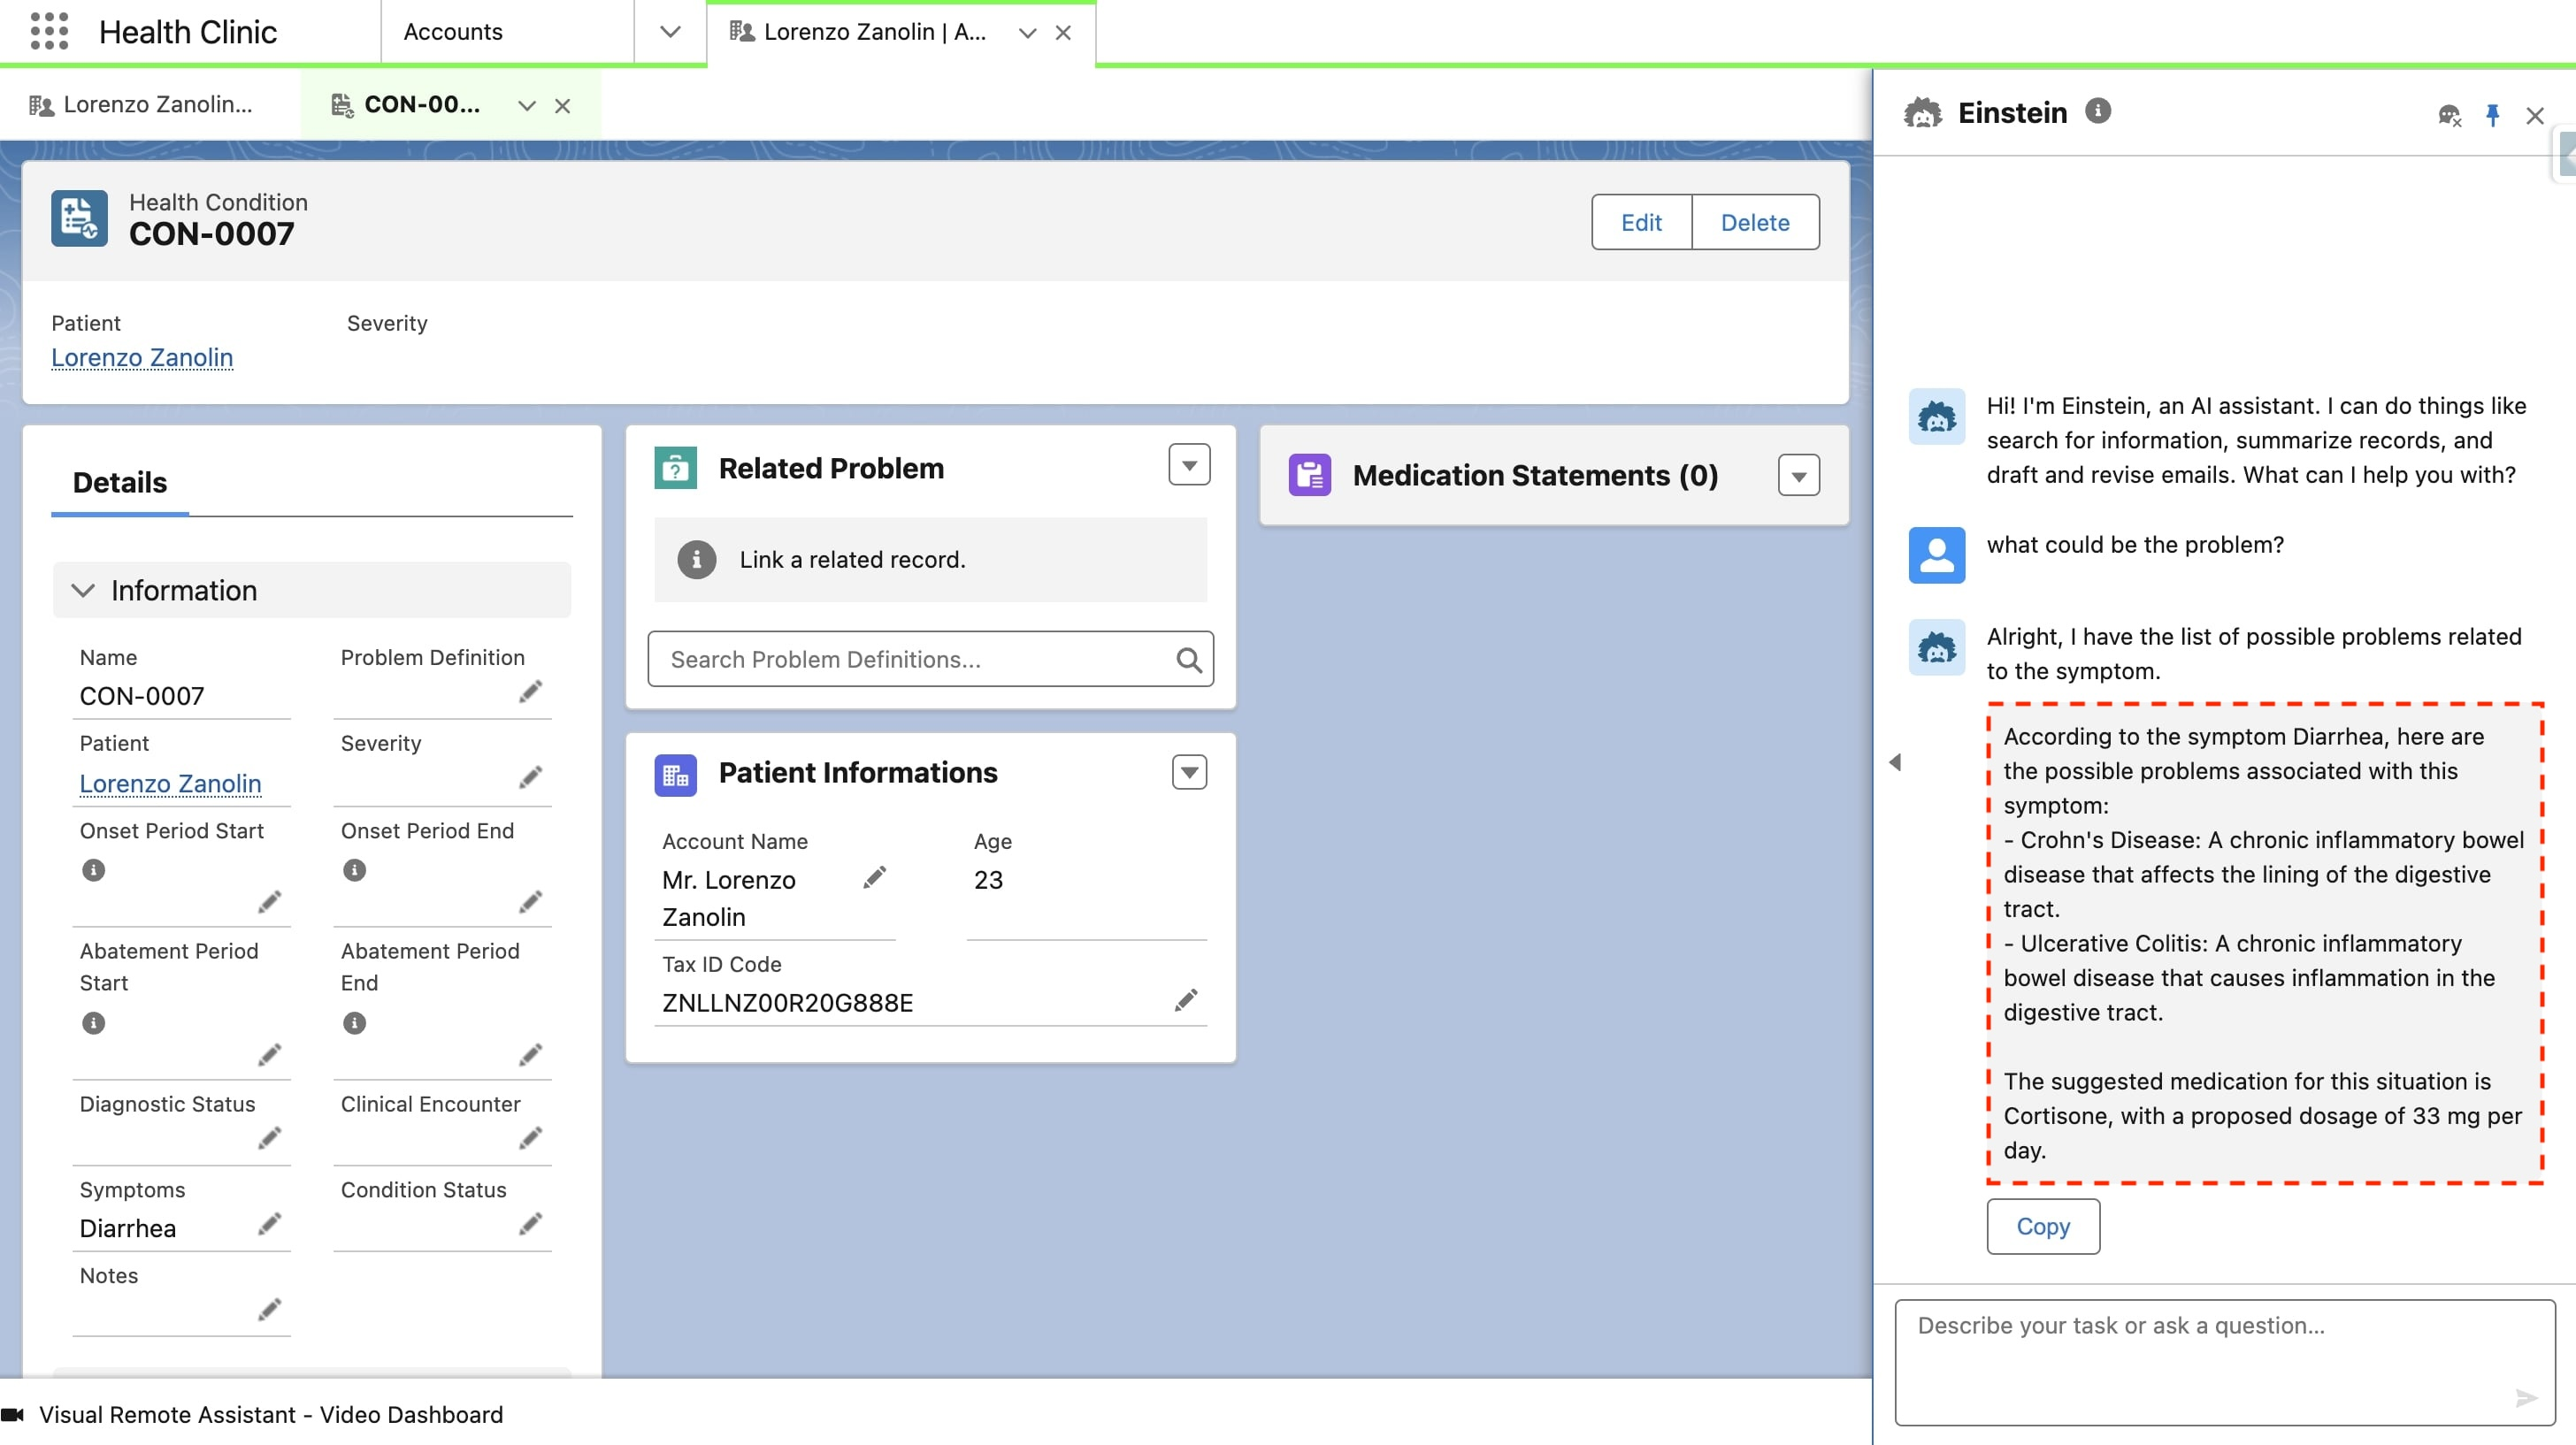
\includegraphics[scale=0.1]{images/ListPossibleProblems.jpg}
\end{figure}}
\end{frame}

\begin{frame}{Send Visit Details}
  
  \only<1->{Creates a draft email summarizing the patient’s latest Clinical Encounter for the doctor to review and edit.}

  \uncover<2->{\begin{figure}[b]
    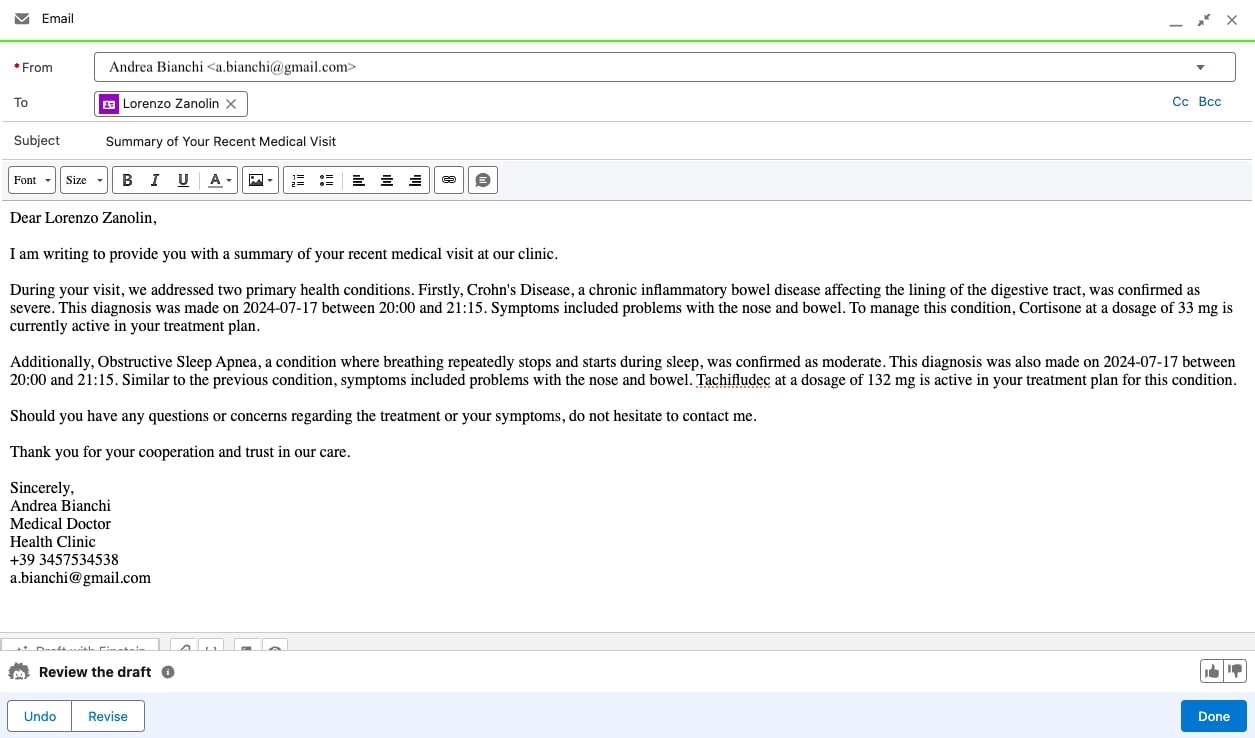
\includegraphics[scale=0.22]{images/SendPatientDetails.jpg}
\end{figure}}
\end{frame}

\begin{frame}{Evaluation Framework}
  
  \only<1->{For each task, the output of each model was evaluated in comparison to the clinician’s notes.\\}
  \vspace{2mm}
  \uncover<2->{
    \textbf{Automatic Evaluation}: 
    \begin{itemize}
      \item Metrics: ROUGE, BLEU, METEOR, Word2Vec and BERTScore.
    \end{itemize}
  }
  \vspace{2mm}
  \uncover<3->{
    \textbf{Human Evaluation}: 
    \begin{itemize}
      \item A sample of 20 physicians tested the system, providing feedback via a Likert scale (1-5) on four aspects: 
      \begin{itemize}
        \item Accuracy: alignment with clinician notes
        \item Relevance: appropriateness to the query
        \item Coverage: completeness of information
        \item Clarity: syntax and overall quality
      \end{itemize}
    \end{itemize}
  }
\end{frame}

\begin{frame}{Evaluation Framework - cont'd}
  \textbf{G-Eval Evaluation}: 
  \begin{itemize}
    \item Framework used to evaluate model outputs, consistently using the clinician’s notes as a reference.
    \item Compared against human evaluation.
  \end{itemize}

  \begin{figure}[b]
    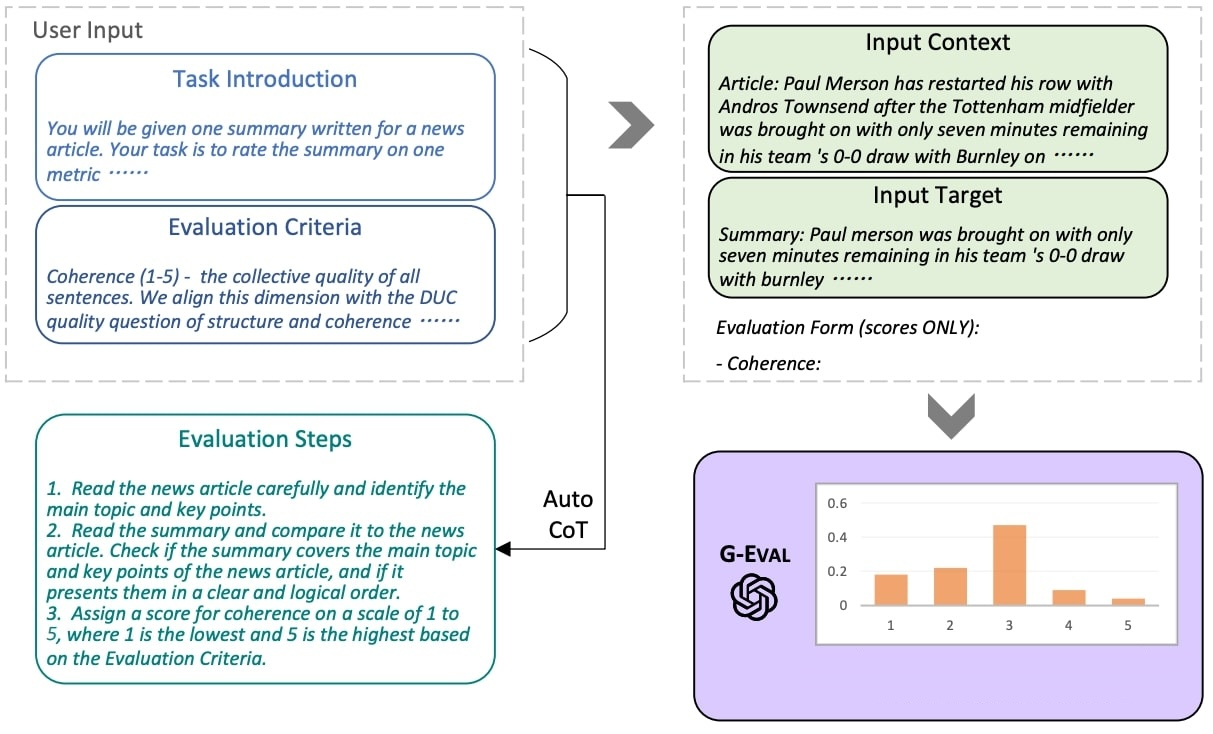
\includegraphics[scale=0.18]{images/G-Eval.jpg}
  \end{figure}

\end{frame}

\begin{frame}[shrink=32]{Automatic Evaluation}
  
  \vspace{10mm}
  \centering
  \begin{threeparttable}[c]
    \setlength{\extrarowheight}{2pt}
    %\caption{Automatic Metrics evaluated over the outputs of the various models.}
    \begin{tabular}{|l|c|c|c|c|c|c|c|}
    \hline
    Model & Rouge1 & Rouge2 & RougeL & BLEU & METEOR & Word2Vec & BERTscore \\
    \hline
    \multicolumn{8}{|c|}{\textbf{Patient Summary}} \\
    \hline
    GPT4      & 0.3966 & 0.1139 & 0.2380 & 0.1470 & 0.2198 & 0.9035 & 0.8458 \\
    GPT4 32k  & 0.3963 & 0.1043 & 0.2439 & 0.1742 & 0.2349 & \textbf{0.9150} & 0.8428 \\
    \textbf{GPT4 Omnni}     & \textbf{0.4286} & \textbf{0.1438} & \textbf{0.2857} & \textbf{0.2013} & \textbf{0.2692} & 0.8987 & \textbf{0.8572} \\
    Anthropic & 0.3761 & 0.1073 & 0.2222 & 0.1054 & 0.1905 & 0.8702 & 0.8504 \\
    \hline
    \multicolumn{8}{|c|}{\textbf{List Possible Problems}} \\
    \hline
    \textbf{GPT4}      & \textbf{0.4444} & \textbf{0.1649} & \textbf{0.3838} & 0.1851 & \textbf{0.3690} & 0.8496 & \textbf{0.9007} \\
    GPT4 32k  & 0.4228 & 0.1322 & 0.2927 & \textbf{0.2180} & 0.2726 & \textbf{0.8819} & 0.8881 \\
    GPT4 Omni     & 0.3800 & 0.0612 & 0.2600 & 0.1366 & 0.2709 & 0.8529 & 0.8789 \\
    Anthropic & 0.3579 & 0.0645 & 0.2526 & 0.1221 & 0.2480 & 0.8325 & 0.8810 \\
    \hline
    \multicolumn{8}{|c|}{\textbf{Email Generation}} \\
    \hline
    GPT4      & 0.3697 & 0.0845 & 0.2129 & 0.1704 & 0.2991 & 0.9164 & 0.8510 \\
    GPT4 32k  & 0.3371 & 0.0460 & 0.1771 & 0.1153 & 0.2811 & 0.8801 & 0.8443 \\
    \textbf{GPT4 Omni}     & \textbf{0.4536} & \textbf{0.1295} & \textbf{0.2526} & \textbf{0.2345} & \textbf{0.3605} & \textbf{0.9295} & 0.8735 \\
    Anthropic & 0.4375 & 0.1166 & 0.2321 & 0.2037 & 0.3037 & 0.9219 & \textbf{0.8739} \\
    \hline
    \end{tabular}
  \end{threeparttable}
\end{frame}

\begin{frame}{Human Evaluation}
  Mean and standard deviation of Human Evaluation scores.\\
  %\vspace{10mm}
  {\tiny
  \centering
  \begin{table}[]
    \setlength{\extrarowheight}{2pt}
    \begin{tabular}{|l|c|c|c|c|}
    \hline
    Model & Accuracy & Relevance & Coverage & Clarity  \\
    \hline
    \multicolumn{5}{|c|}{\textbf{Patient Summary}} \\
    \hline
    GPT4     & $\mathbf{\mu=3.83}$, $\mathbf{\sigma=0.62}$ & $\mu=3.72$, $\sigma=0.75$ & $\mu=3.06$, $\sigma=0.73$ & $\mu=3.83$, $\sigma=0.71$ \\
    GPT4 32k  & $\mu=3.72$, $\sigma=0.67$ & $\mathbf{\mu=3.78}$, $\mathbf{\sigma=0.81}$ & $\mu=3.22$, $\sigma=0.94$ & $\mathbf{\mu=4.06}$, $\mathbf{\sigma=0.54}$ \\
    GPT4 Omni & $\mu=3.83$, $\sigma=0.86$ & $\mu=3.50$, $\sigma=1.10$ & $\mu=3.33$, $\sigma=0.77$ & $\mu=3.89$, $\sigma=0.76$ \\
    \textbf{Anthropic} & $\mu=3.83$, $\sigma=1.04$ & $\mu=3.83$, $\sigma=0.99$ & $\mathbf{\mu=3.67}$, $\mathbf{\sigma=0.59}$ & $\mu=4.17$, $\sigma=0.86$ \\
    \hline
    \multicolumn{5}{|c|}{\textbf{List Possible Problems}} \\
    \hline
    GPT4      & $\mathbf{\mu=3.95}$, $\mathbf{\sigma=0.87}$ & $\mu=4.00$, $\sigma=0.84$ & $\mu=3.61$, $\sigma=0.85$ & $\mathbf{\mu=3.94}$, $\mathbf{\sigma=0.73}$ \\
    GPT4 32k  & $\mu=3.83$, $\sigma=0.79$ & $\mu=3.94$, $\sigma=0.73$ & $\mu=3.50$, $\sigma=0.86$ & $\mu=4.17$, $\sigma=0.79$ \\
    \textbf{GPT4 Omni}     & $\mu=3.90$, $\sigma=1.08$ & $\mu=4.00$, $\sigma=0.97$ & $\mu=3.72$, $\sigma=1.02$ & $\mu=4.05$, $\sigma=0.80$ \\
    Anthropic & $\mu=3.90$, $\sigma=0.90$ & $\mathbf{\mu=4.06}$, $\mathbf{\sigma=0.80}$ & $\mu=3.72$, $\sigma=1.02$ & $\mu=3.94$, $\sigma=0.94$ \\
    \hline
    \multicolumn{5}{|c|}{\textbf{Email Generation}} \\
    \hline
    GPT4      & $\mu=3.17$, $\sigma=0.98$ & $\mu=3.22$, $\sigma=0.88$ & $\mu=2.94$, $\sigma=0.99$ & $\mu=3.28$, $\sigma=0.89$ \\
    GPT4 32k  & $\mu=3.00$, $\sigma=1.08$ & $\mu=3.56$, $\sigma=0.92$ & $\mu=3.33$, $\sigma=1.00$ & $\mu=3.44$, $\sigma=1.20$ \\
    GPT4 Omni     & $\mu=3.78$, $\sigma=0.94$ & $\mathbf{\mu=4.06}$, $\mathbf{\sigma=0.64}$ & $\mathbf{\mu=3.72}$, $\mathbf{\sigma=0.67}$ & $\mu=3.94$, $\sigma=0.94$ \\
    \textbf{Anthropic} & $\mu=4.06$, $\sigma=0.80$ & $\mu=4.11$, $\sigma=0.76$ & $\mu=3.90$, $\sigma=0.90$ & $\mu=4.06$, $\sigma=0.97$ \\
    \hline
  \end{tabular}
\end{table}
}
\end{frame}

\begin{frame}{Human Evaluation - cont'd}
  \textbf{Inter-rater agreement}\\
  for all pairs of raters 
  \[
  P=\{\{R_i= [r_{i,1}, \ldots, r_{i,n}],R_j = [r_{j,1},\ldots,r_{j,n}]\}|R_i,R_j\in R, R_i\neq R_j\}
  \]
  the corresponding $\kappa_{w_{i,j}}$ values were calculated.\\
  Subsequently, the average $\kappa_w = \frac{1}{|P|}\sum_{(i,j)\in P} \kappa_{w_{i,j}}$ was computed.
  \vspace{5mm}
  {\tiny
  \begin{table}[b]
    \centering
    \setlength{\extrarowheight}{2pt}
    \begin{tabular}{|c|c|c|c|}
    \hline
    GPT4 & GPT4 32K & GPT4 Omni & Anthropic\\
    \hline
    \multicolumn{4}{|c|}{\textbf{Patient Summary}} \\
    \hline
    $\kappa_w=0.25$ & $\kappa_w=0.29$ & $\kappa_w=0.37$ & $\kappa_w=0.52$ \\
    \hline
    \multicolumn{4}{|c|}{\textbf{List Possible Problems}} \\
    \hline
    $\kappa_w=0.61$ & $\kappa_w=0.63$ & $\kappa_w=0.63$ & $\kappa_w=0.57$ \\
    \hline
    \multicolumn{4}{|c|}{\textbf{Email Generation}} \\
    \hline
    $\kappa_w=0.53$ & $\kappa_w=0.61$ & $\kappa_w=0.69$ & $\kappa_w=0.72$ \\
    \hline
    \end{tabular}
  \end{table}
  }
\end{frame}

\begin{frame}{G-Eval Evaluation}
  \centering
  Comparison of each metric between G-Eval and Human scores.
  \vspace{5mm}
  \begin{figure}[b]
    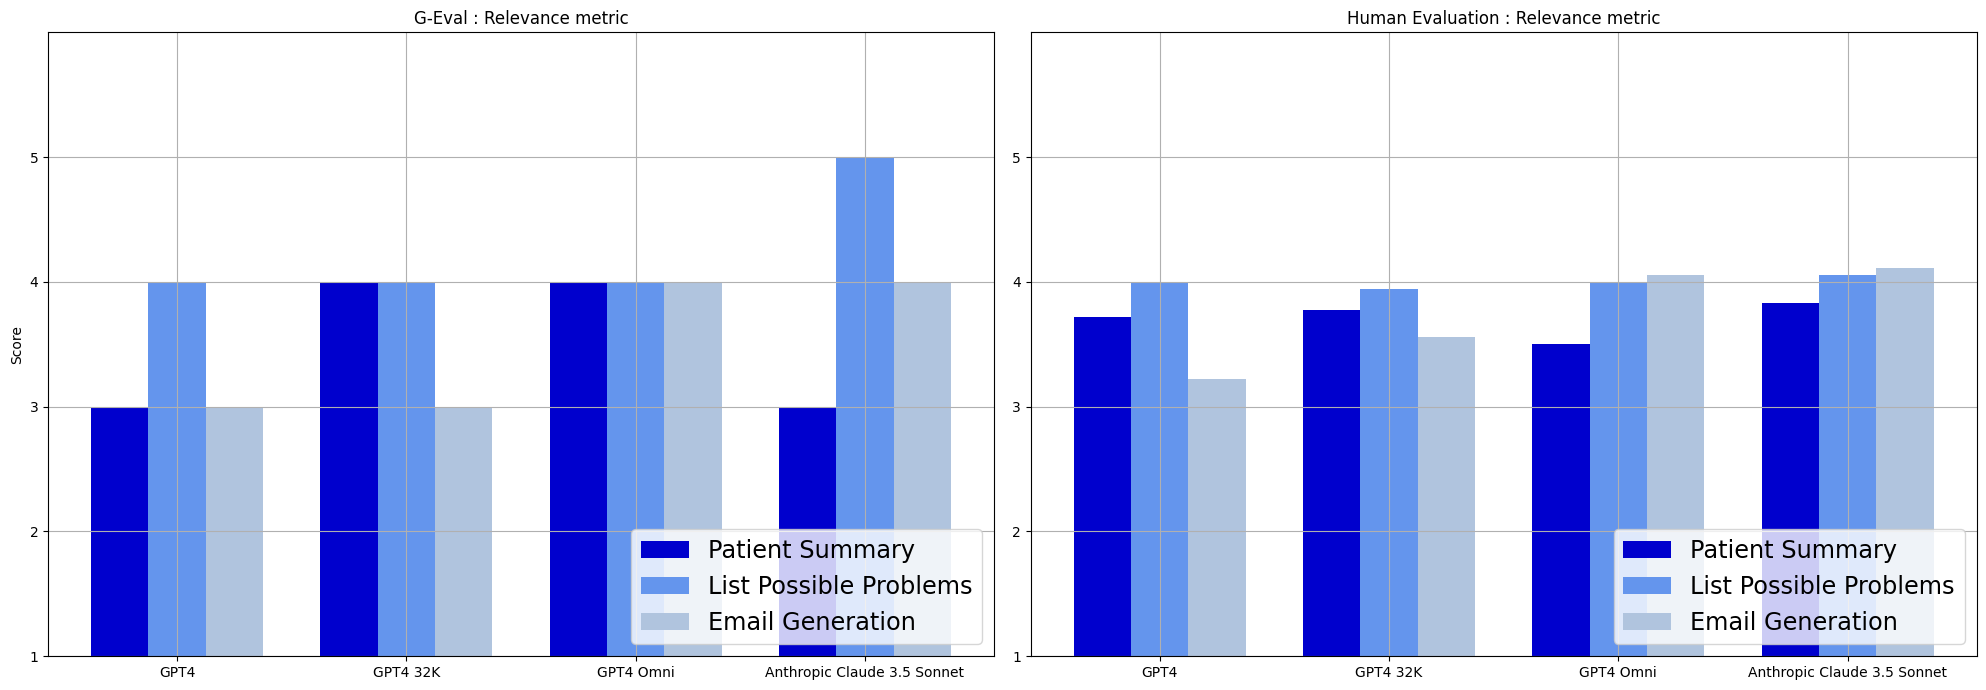
\includegraphics[width=\textwidth]{images/comparison.png}
  \end{figure}  
\end{frame}

\begin{frame}{Conclusions}
  
  \only<1->{
    \textbf{Results}\\
    \begin{itemize}
      \item Generative AI can increase productivity
      \item New proposed framework that includes human and automatic evaluation
      \begin{itemize}
        \item Sematical metrics work better in this context
        \item Raters gave similar scores to shorter text
      \end{itemize}
    \end{itemize}
  }
    \vspace{5mm}
  \uncover<2->{
    \textbf{Future Directions}
    \begin{itemize}
      \item Conduct a number of measurements with G-Eval equal to the number of raters to compare G-Eval with Human Feedback.
    \end{itemize}
  }

\end{frame}

%\begin{frame}[allowframebreaks, noframenumbering]{References}
%\bibliography{bibliography}
%\bibliographystyle{plain}
%\hfill
%\end{frame}
\end{document}